Bảng~\ref{tab:ablation} và Hình~\ref{fig:features} cho kết quả bỏ hoặc thêm nhóm ở 8 trường hợp (4 bộ $\times$ 2 mức nhãn), Bảng~\ref{tab:perm} cho độ quan trọng hoán vị của mô hình đủ 17 đầu vào.

\paragraph{Biến thời gian $t$.} Bỏ $t$ làm sai số tăng có ý nghĩa ở 6 trên 8 trường hợp, nhiều nhất 1{,}35 lần; trường hợp duy nhất có lợi là MIT 10\,\% (tỉ số 0{,}90). Ngược lại, chỉ dùng $t$ mà bỏ hết đặc trưng sạc cho sai số gấp 1{,}20--12{,}33 lần: tuổi của cell một mình không đủ để biết SOH, vì các cell già đi với tốc độ rất khác nhau (tuổi thọ trong mỗi bộ chênh nhau nhiều lần, Bảng~\ref{tab:datastats}). Hoán vị $t$ giữa các hàng test làm sai số tăng 1{,}47--8{,}10 lần, nên mô hình thật sự dùng biến này.

\paragraph{Ba nhóm đặc trưng sạc.} Không có trường hợp nào bỏ một nhóm mà sai số giảm có ý nghĩa. Nhóm V (điện áp pha CC) và nhóm QT (điện lượng, thời gian) mang nhiều thông tin nhất: bỏ nhóm V làm sai số tăng có ý nghĩa ở 6 trên 8 trường hợp, bỏ nhóm QT ở 4 trên 8, có trường hợp gần gấp đôi (1{,}99). Bỏ nhóm I (dòng điện pha CV) chỉ làm sai số tăng có ý nghĩa ở 2 trường hợp. Chỉ giữ nhóm QT và $t$, tức 5 đầu vào, kém bộ đầy đủ có ý nghĩa ở 6 trên 8 trường hợp. Phép hoán vị cho cùng nhận xét: hoán vị nhóm QT làm sai số tăng tới 18{,}82 lần, nhóm V tới 5{,}02 lần, nhóm I chỉ tới 3{,}00 lần.

\paragraph{Chọn đặc trưng tự động.} Khi bỏ các đầu vào mà hoán vị trên validation làm sai số tăng dưới 1\,\%, mỗi fold giữ lại trung vị 7--17 trên 17 đầu vào tuỳ bộ và mức nhãn; hay bị bỏ nhất là trung bình dòng điện, độ lệch chuẩn dòng điện và độ lệch chuẩn điện áp. Trên test, cách chọn này cho sai số bằng 0{,}99--1{,}02 lần bộ đầy đủ, không khác có ý nghĩa ở trường hợp nào, tức bớt đầu vào không làm mô hình tốt lên.

\paragraph{Đọc kết quả.} Mọi tập rút gọn đều kém bộ đầy đủ ở ít nhất một trường hợp, và các trường hợp có lợi (bỏ $t$ ở MIT 10\,\%; thêm 16 đặc trưng tương đối ở TJU 70\,\%) không lặp lại ở bộ khác. Chọn đầu vào riêng cho từng bộ dựa trên những kết quả này là chọn mô hình trên tập test, còn chọn riêng cho từng fold bằng validation thì không cải thiện. Vì vậy đồ án dùng chung bộ 17 đầu vào cho mọi bộ dữ liệu và mọi mô hình.

\begin{table}[!htbp]\centering\small\setlength{\tabcolsep}{4pt}
\caption[Bỏ hoặc thêm nhóm đầu vào với GBDT]{Bỏ hoặc thêm nhóm đầu vào, GBDT trên đúng các fold không rò rỉ (3 lần lặp $\times$ 5 fold). Hàng đầu: MAE theo cell ($\times10^{-3}$) với đủ 17 đầu vào. Các hàng sau: tỉ số MAE so với đủ 17 đầu vào. $^{*}$/$^{\dagger}$: thấp hơn/cao hơn có ý nghĩa (Wilcoxon ghép cặp theo cell, Holm qua bốn bộ).}\label{tab:ablation}
\begin{adjustbox}{max width=\textwidth}\begin{tabular}{lrrrrrrrr}\toprule
 & \multicolumn{2}{c}{XJTU} & \multicolumn{2}{c}{TJU} & \multicolumn{2}{c}{MIT} & \multicolumn{2}{c}{HUST} \\\cmidrule(lr){2-3}\cmidrule(lr){4-5}\cmidrule(lr){6-7}\cmidrule(lr){8-9}
Tập đầu vào & 10\,\% & 70\,\% & 10\,\% & 70\,\% & 10\,\% & 70\,\% & 10\,\% & 70\,\% \\\midrule
đủ 17 đầu vào (MAE) & 14{,}01 & 9{,}64 & 12{,}60 & 6{,}96 & 3{,}15 & 1{,}59 & 23{,}84 & 14{,}60 \\
\addlinespace[2pt]
bỏ $t$ & 1{,}12$^{\dagger}$ & 1{,}18$^{\dagger}$ & 1{,}32$^{\dagger}$ & 1{,}11$^{\dagger}$ & 0{,}90$^{*}$ & 1{,}01 & 1{,}30$^{\dagger}$ & 1{,}35$^{\dagger}$ \\
chỉ $t$ & 1{,}92$^{\dagger}$ & 2{,}67$^{\dagger}$ & 1{,}75$^{\dagger}$ & 3{,}03$^{\dagger}$ & 6{,}55$^{\dagger}$ & 12{,}33$^{\dagger}$ & 1{,}20$^{\dagger}$ & 1{,}86$^{\dagger}$ \\
bỏ nhóm V & 0{,}99 & 1{,}06$^{\dagger}$ & 1{,}03$^{\dagger}$ & 1{,}10$^{\dagger}$ & 1{,}02 & 1{,}16$^{\dagger}$ & 1{,}11$^{\dagger}$ & 1{,}32$^{\dagger}$ \\
bỏ nhóm I & 0{,}96 & 1{,}03 & 1{,}06$^{\dagger}$ & 1{,}05 & 1{,}00 & 1{,}00 & 1{,}01 & 1{,}06$^{\dagger}$ \\
bỏ nhóm QT & 1{,}05$^{\dagger}$ & 1{,}02$^{\dagger}$ & 1{,}00 & 1{,}00 & 1{,}73$^{\dagger}$ & 1{,}99$^{\dagger}$ & 1{,}01 & 1{,}02 \\
chỉ QT và $t$ & 0{,}96 & 1{,}12$^{\dagger}$ & 1{,}15$^{\dagger}$ & 1{,}33$^{\dagger}$ & 1{,}05 & 1{,}26$^{\dagger}$ & 1{,}17$^{\dagger}$ & 1{,}52$^{\dagger}$ \\
thêm 16 đặc trưng tương đối & 1{,}02 & 0{,}99 & 0{,}98 & 0{,}89$^{*}$ & 1{,}19$^{\dagger}$ & 1{,}14$^{\dagger}$ & 1{,}03 & 0{,}95 \\
chọn trên validation & 1{,}00 & 1{,}01 & 1{,}01 & 0{,}99 & 1{,}00 & 1{,}00 & 1{,}02 & 1{,}00 \\
thêm $1/T$ (chỉ TJU) & -- & -- & 0{,}99$^{*}$ & 1{,}00 & -- & -- & -- & -- \\
\bottomrule\end{tabular}\end{adjustbox}\end{table}

\begin{table}[!htbp]\centering\small\setlength{\tabcolsep}{4pt}
\caption[Độ quan trọng hoán vị trên test]{Độ quan trọng hoán vị trên test của GBDT đủ 17 đầu vào: tỉ số MAE theo cell khi hoán vị cả một nhóm (hoặc một đầu vào) giữa các hàng test so với khi không hoán vị, trung bình 15 fold. Bằng 1: mô hình không dùng thông tin của nhóm đó.}\label{tab:perm}
\begin{adjustbox}{max width=\textwidth}\begin{tabular}{lrrrrrrrr}\toprule
 & \multicolumn{2}{c}{XJTU} & \multicolumn{2}{c}{TJU} & \multicolumn{2}{c}{MIT} & \multicolumn{2}{c}{HUST} \\\cmidrule(lr){2-3}\cmidrule(lr){4-5}\cmidrule(lr){6-7}\cmidrule(lr){8-9}
Hoán vị & 10\,\% & 70\,\% & 10\,\% & 70\,\% & 10\,\% & 70\,\% & 10\,\% & 70\,\% \\\midrule
nhóm V (6) & 1{,}29 & 1{,}76 & 1{,}30 & 2{,}39 & 3{,}37 & 5{,}02 & 1{,}18 & 2{,}10 \\
nhóm I (6) & 1{,}32 & 1{,}77 & 1{,}83 & 3{,}00 & 1{,}14 & 1{,}70 & 1{,}12 & 1{,}68 \\
nhóm QT (4) & 2{,}16 & 2{,}59 & 1{,}30 & 1{,}98 & 8{,}41 & 18{,}82 & 1{,}40 & 1{,}93 \\
$t$ & 1{,}47 & 2{,}77 & 4{,}59 & 8{,}10 & 1{,}78 & 2{,}61 & 2{,}88 & 4{,}27 \\
\bottomrule\end{tabular}\end{adjustbox}\end{table}

\begin{figure}[!htbp]\centering
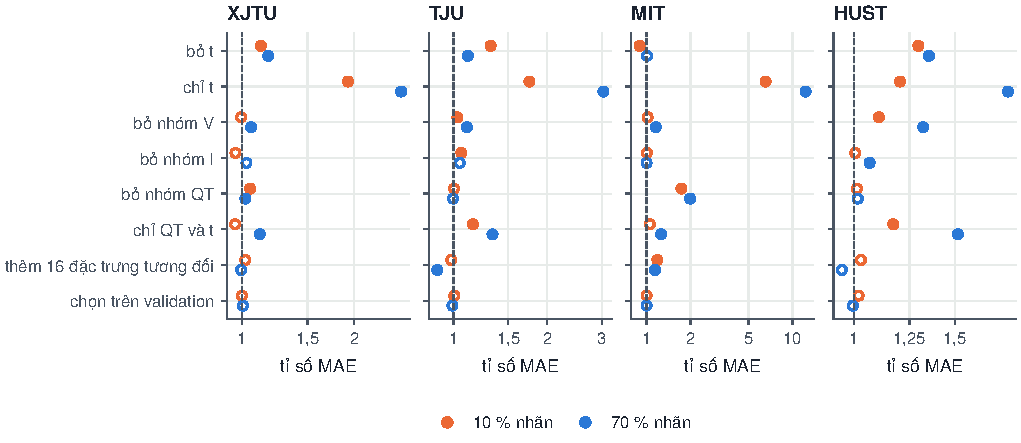
\includegraphics[width=\textwidth]{graphics/fig_features.pdf}
\caption[Bỏ hoặc thêm nhóm đầu vào: tỉ số MAE so với đủ 17 đầu vào]{Tỉ số MAE theo cell so với GBDT đủ 17 đầu vào, theo tập đầu vào và mức nhãn (thang log). Điểm đặc: khác có ý nghĩa (Wilcoxon theo cell, Holm qua bốn bộ); điểm rỗng: không có ý nghĩa. Vạch đứt: bằng bộ đầy đủ.}\label{fig:features}
\end{figure}
